\documentclass[../practica.root.tex]{subfiles}

\begin{document}
\begin{enumerate}
    \item Dado $A = \{1, 2, 3\}$, indicar V ó F:
          \begin{enumerate}
              \item $1 \in A$ \cmark
              \item $\{1\} \subseteq A$ \cmark
              \item $\{2, 1\} \subseteq A$ \cmark
              \item $\{1, 3\} \in A$ \xmark
              \item $\{2\} \in A$ \xmark
          \end{enumerate}

    \item Dado $A = \{1, 2, \{3\}, \{1, 2\}\}$, indicar V ó F
          \begin{enumerate}
              \item $3 \in A$ \xmark
              \item $\{3\} \subseteq A$ \xmark
              \item $\{3\} \in A$ \cmark
              \item $\{\{3\}\} \subseteq A$ \cmark
              \item $\{1, 2\} \in A$ \cmark
              \item $\{1, 2\} \subseteq A$ \cmark
              \item $\{\{1, 2\}\} \subseteq A$ \cmark
              \item $\{\{1, 2\}, 3\} \subseteq A$ \xmark
              \item $\emptyset \in A$ \xmark
              \item $\emptyset \subseteq A$ \cmark
              \item $A \in A$ \xmark
              \item $A \subseteq A$ \cmark
          \end{enumerate}

    \item Determinar si $A \subseteq B$
          \begin{enumerate}
              \item $A = \{1, 2, 3\}$, $B = \{5, 4, 3, 2, 1\}$ \cmark
              \item $A = \{1, 2, 3\}$, $B = \{1, 2, \{3\}, -3\}$ \xmark
              \item $A = \{x \in \R / 2 < |x| < 3\}$, $B = \{x \in \R / x^2 < 3\}$ \xmark
              \item $A = \{\emptyset\}$, $B = \emptyset$ \xmark
          \end{enumerate}

    \item Describir por comprensión usando \textit{solo una} ecuación
          \begin{enumerate}
              \item
                    \[ \{-3, 1, 5\} = \{x \in \N / (x+3)(x-1)(x-5) = 0\} \]
                    \[ (-\infty, 2]\cup[7, +\infty) = \{x \in \R /  x < 2 \lor x > 7  \}\]
              \item
                    \begin{enumerate}
                        \item $\{(x; y) \in \R^2 / x = y\}$
                        \item $\{(x; y) \in \R^2 / -x = y\}$
                        \item $\{(x; y) \in \R^2 / |x| = |y|\}$
                        \item $\{(x; y) \in \R^2 / |x| = 2\}$
                        \item $\{(x; y) \in \R^2 / x = -1\}$
                        \item $\{(x; y) \in \R^2 / y < 0\}$
                    \end{enumerate}
          \end{enumerate}

    \item Dados $A = \{1, -2, 7, 3\}$, $B = \{1, \{3\}, 10\}$ y $C = \{-2, \{1, 2, 3\}, 3\}$, y
          $U = \{1, \{3\}, -2, 7, 10, \{1,2,3\},3\}$, hallar
          \begin{enumerate}
              \item $A \cap (B \triangle C)$
                    \[ B \triangle C = \{1, \{3\}, 10, -2 , \{1, 2, 3\}, 3\} \]
                    \begin{align*}
                        A \cap (B \triangle C) & = \{1, -2, 7, 3\}\cap\{1, \{3\}, 10, -2 , \{1, 2, 3\}, 3\} \\
                                               & = \boxed{\{1, -2, 3\}}
                    \end{align*}

              \item $(A \cap B)\triangle(A \cap C)$
                    \begin{align*}
                        A \cap B & =  \{1, -2, 7, 3\} \cap \{1, \{3\}, 10\} = \{1\}         \\
                        A \cap C & = \{1, -2, 7, 3\} \cap \{-2, \{1, 2, 3\}, 3\} = \{-2,3\}
                    \end{align*}
                    \[ \{1\} \triangle \{-2,3\} = \boxed{\{1, -2, 3\}}\]

              \item $A^c \cap B^c \cap C^c$
                    \begin{align*}
                        A^c & = \{\{3\}, 10, \{1, 2, 3\}\} \\
                        B^c & = \{-2, 7, \{1, 2, 3\}, 3\}  \\
                        C^c & = \{1, \{3\}, 7, 10\}
                    \end{align*}
                    \[ \{\{3\}, 10, \{1, 2, 3\}\} \cap \{-2, 7, \{1, 2, 3\}, 3\} \cap \{1, \{3\}, 7, 10\} \]
                    \[ \{ \{1, 2, 3\} \} \cap \{1, \{3\}, 7, 10\} = \boxed{\emptyset} \]
          \end{enumerate}

    \item Dados $A, B, C \subseteq V$, describir:
          \begin{enumerate}
              \item $(A \cup B \cup C)^c$ como intersecciones y complementos
                    \[ \boxed{A^c \cap B^c \cap C^c} \]
              \item $(A \cap B \cap C)^c$ como uniones y complementos
                    \[ \boxed{A^c \cup B^c \cup C^c} \]
          \end{enumerate}

    \item Representar en un diagrama de Venn: \\
          \begin{enumerate}
              \item $(A \cup B^c) \cap C$
              \item $A \triangle (B \cup C)$
              \item $(A \cup (B \triangle C)$
          \end{enumerate}
          \begin{figure}[h]
              \centering
              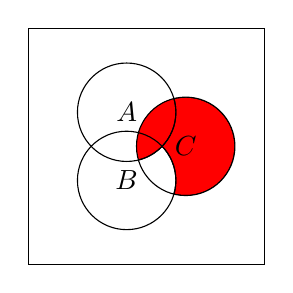
\begin{tikzpicture}[scale=0.5]
                  \draw (-3,-3) rectangle (3,3);
                  \begin{scope}[draw=transparent]
                      \clip (360:1) circle[radius=1.25];
                      \draw[fill=red] (360:1) circle[radius=1.25];
                      \draw[fill=white] (240:1) circle[radius=1.25];
                      \draw[fill=red] (120:1) circle[radius=1.25];
                  \end{scope}

                  \draw (120:1) node{$A$} circle[radius=1.25];
                  \draw (240:1) node{$B$} circle[radius=1.25];
                  \draw (360:1) node{$C$} circle[radius=1.25];
              \end{tikzpicture}
              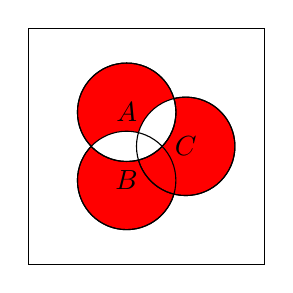
\begin{tikzpicture}[scale=0.5]
                  \draw (-3,-3) rectangle (3,3);

                  \begin{scope}[draw=transparent]
                      \draw[fill=red] (240:1) circle[radius=1.25];
                      \draw[fill=red] (360:1) circle[radius=1.25];
                      \draw[fill=red] (120:1) circle[radius=1.25];
                      \clip (240:1) circle[radius=1.25] (360:1) circle[radius=1.25];
                      \draw[fill=white] (120:1) circle[radius=1.25];
                  \end{scope}

                  \draw (120:1) node{$A$} circle[radius=1.25];
                  \draw (240:1) node{$B$} circle[radius=1.25];
                  \draw (360:1) node{$C$} circle[radius=1.25];
              \end{tikzpicture}
              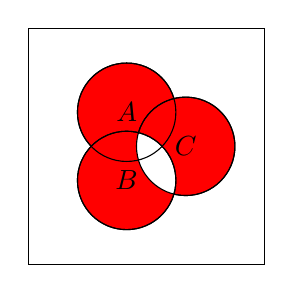
\begin{tikzpicture}[scale=0.5]
                  \draw (-3,-3) rectangle (3,3);
                  \begin{scope}[draw=transparent]
                      \draw[fill=red] (120:1) circle[radius=1.25];
                      \draw[fill=red] (360:1) circle[radius=1.25];
                      \draw[fill=red] (240:1) circle[radius=1.25];
                      \clip (360:1) circle[radius=1.25];
                      \clip (240:1) circle[radius=1.25];
                      \draw[fill=white] (240:1) circle[radius=1.25];
                  \end{scope}
                  %\draw[fill=red] (120:1) circle[radius=1.25];

                  \draw (120:1) node{$A$} circle[radius=1.25];
                  \draw (240:1) node{$B$} circle[radius=1.25];
                  \draw (360:1) node{$C$} circle[radius=1.25];
              \end{tikzpicture}
          \end{figure}

    \item Encontrar fórmulas que describan los siguientes diagramas de Venn, usando solo $\cup$, $\cap$ y $^c$
          \begin{enumerate}
              \item
                    \[ A - B = A \cap B^c \]
                    \[ (B \cap C) - A = (B \cap C) \cap A^c \]
                    \[ \boxed{(A \cap B^c) \cup (B \cap C \cap A^c)} \]
              \item
                    \[ A \triangle B = (A \cup C) - (A \cap C) = (A \cup C) \cap (A \cap C)^c \]
                    \[ (A \cup C) \cap (A \cap C)^c - B = \boxed{(A \cup C) \cap (A \cap C)^c \cap B^c} \]
              \item
                    \[ (A \cap B) \cup (B \cap C) \cup (C \cap A) \]
                    \[ (A \cap B) \cup (B \cap C) \cup (C \cap A) - (A \cap B \cap C) \]
                    \[ \boxed{(A \cap B) \cup (B \cap C) \cup (C \cap A) \cap (A \cap B \cap C)^c} \]
          \end{enumerate}

    \item 9lol

    \item 10lol

\end{enumerate}

\end{document}